\section{Introduction}
Software is becoming increasingly complex and at the same time increasingly safety critical in many domains (e.g., in robotics, autonomous systems such as cars, data-processing software, apps on mobile phones, etc.)
\tom{I do not see the purpose of talking about safety critical here, since this is not the focus at all of your paper...}

To tackle these challenges \note{which ones?}\tom{Indeed...}, developers rely on code reuse and distributed collaborative development tools.
Social coding platforms (\scp)\tom{I do not see a need for the abbreviation SCP. In fact I have never seen this abbreviation used before, meaning it is not a common one. Moreover, the only one you will focus on in this paper is \gh, right?}

 comprise a number of so-called ecosystems\tom{I do not know what is mentioned by "\scp comprise ecosystems"}
  i.e., large collections of interdependent software components that are maintained by large and geographically distributed communities of collaborating contributors~\cite{lungu:2008,decan:2017}.
The ecosystems form large socio-technical networks of technical and social components that interact with each other on top of common software and hardware platforms.
The unprecedented growth of these ecosystems relies on substantial software reuse using different methods and tools \cite{mojica2014large}.
Social coding has substantially improved  both code reuse and collaborative development, providing a huge bazaar of software projects and components that can be reused through explicit project dependencies or forking of software repositories. This is supported by various automated facilities such as pull requests, dependency management tools, issue tracking systems (e.g. \textsf{JIRA}), source code review tools (e.g., \textsf{Gerrit}), Q\&A services (e.g. \textsf{StackOverflow}), continuous integration tools (e.g., \textsf{Travis CI}), and package distribution managers (e.g., \np).

Our research focuses on the phenomenon of forking in particular.
Forking a software repository (referred to as the \textit{mainline}, i.e., the original repository) produces several \textit{forked} repositories.
Two types of forks exist~\cite{Zhou:2020}. \textit{Social forks} are created for isolated development, but with the goal of contributing back to the mainline.
\textit{Variant forks} are created for splitting off a new development branch, often to steer the development into another direction than the mainline, without the intention to contribute back.
Variant forking may split the core development team and always splits the contributing community.
Variant forking creates variants of the mainline repository, which share common code, but also contain variant-specific code that needs to be maintained.
A mainline repository together with all its variant repositories can be seen as a software product family, inspired by the notion of \textit{software product lines}~\cite{berger.ea:2020:emse}.
The  family members have software artefacts in common, but also contain artefacts that are specific to one or multiple variants.

\begin{figure}[ht]
  \begin{center}
  \small
  %\vspace{-10pt}
    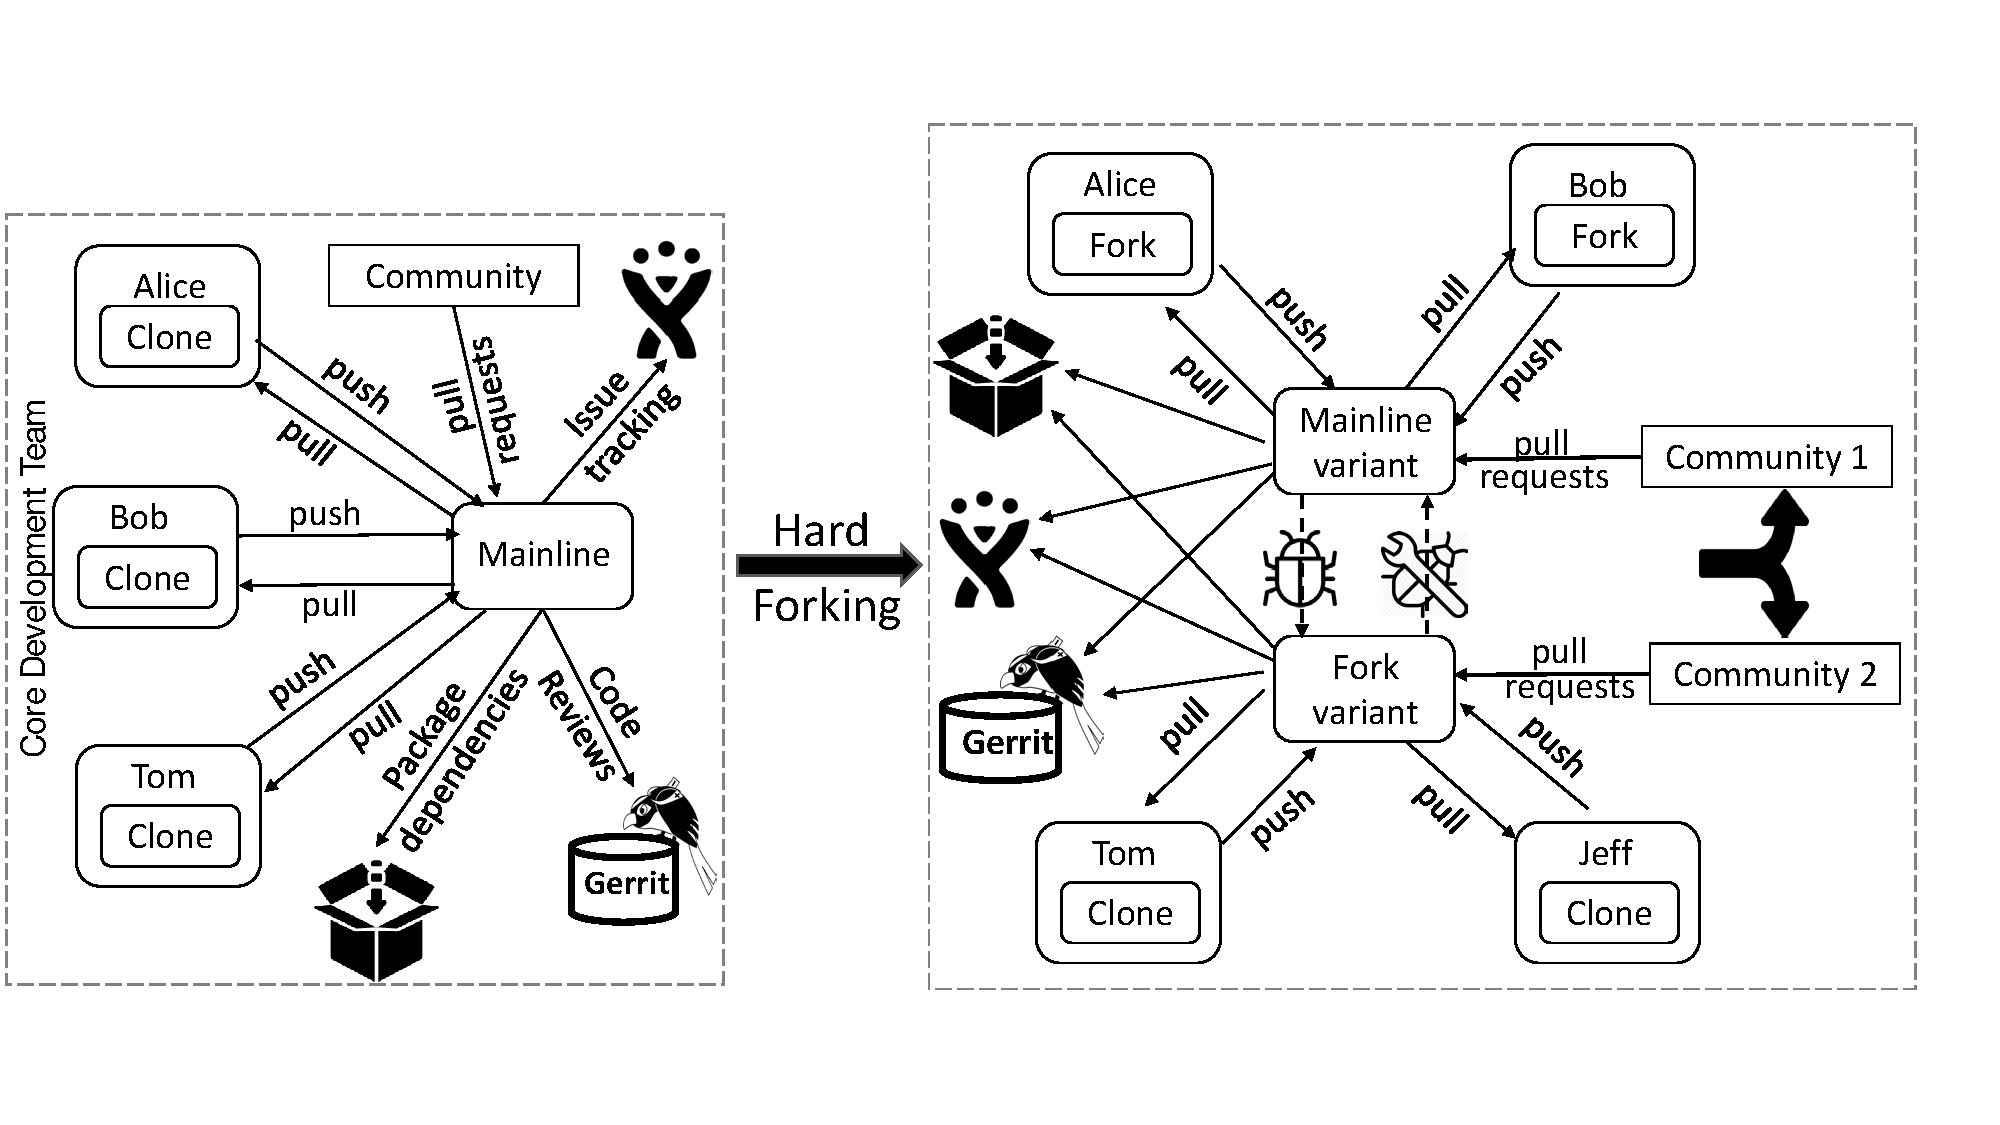
\includegraphics[width=0.5\textwidth]{figures/Collaboration.pdf}
  \end{center}
  \caption{Maintenance of a software repository before (left) and after (right) variant forking.}
  %\vspace{-10pt}
  \label{fig:forking}
\end{figure}

Figure~\ref{fig:forking} illustrates the development activities on a repository before and after variant forking.
On the left, we can see three core developers (Alice, Bob and Tom) that have write access to the mainline repository.\tom{If Alex, Bob and Tom have write access, then why do they have to go through the pull/push mechanism? Isn't it also possible or them to do direct commits?}
The community interacts with the mainline by sending pull requests, submitting issues and conducting change reviews.
After variant forking, shown on the right, the core developers are split into two.
Alice and Bob remain with the original mainline, while Tom is joined by a new developer Jeff to maintain a new fork variant in parallel to the mainline project.
This parallel development between mainline and variant has split the contributing community. New contributors could decide to contribute to the mainline or the variant, for instance depending on which one is more open to accommodate newcomers.
Furthermore, as a result of parallel maintenance, developers in one of the projects may identify and fix bugs in shared artefacts.\tom{Why would there be any shared artefacts if the split/fork is not a social fork?}
These fixes could be propagated to other members of the family to avoid effort duplication.\tom{Why would there be any incentive to propagate fixes if the variant forks are not social forks?}

There have been many studies on variant forks. However, most of these studies were carried out on \texttt{SourceForge}~\cite{Linus:2012Perspectives,Gregorio:2012,Viseur:2012Forks,Linus:2013CodeForking,Laurent:2008,Linus:2011ToFork}, before the advent of social coding platforms such as \gh.
We have found only two studies that investigated variant forks on \gh~\cite{businge2018appfamilies,Zhou:2020}.
While the pre-\gh studies report controversial perceptions around hard forks~\cite{Chua:Forking:2017,Dixion:2009Forks,Ernst:2010,Linus:2011ToFork,Linus:2014Hackers,Raymond:Cathedral:2001},\tom{You introduce the term "hard forks" but this term has not been introduced before...}
According to Zhou et al.~\cite{Zhou:2020} these perceptions have changed with the advent of \gh. Jiang et al.~\cite{Lo:2017} state that, although forking is controversial in traditional open source software (OSS) communities, it is actually encouraged as a built-in feature in \gh. Jiang et al. ~\cite{Lo:2017} further report that developers fork repositories to submit pull requests, fix bugs, add new features and keep copies (social forks).
Zhou et al.~\cite{Zhou:2020} also report that many variant forks actually start as social forks.

While numerous studies have investigated variant forking, we are not aware of any study that has investigated the socio-technical specificities of these variant forks.
Our research therefore aims at empirically studying the evolution of \textbf{software families} composed of variant project repositories by investigating their socio-technical aspects.
For the social aspects, it would be interesting to look at the interaction and collaboration between communities involved in the mainline and variants.
How different are collaborations with respect to who forked and how the fork has been created?
For the technical aspects, as an example, considering the dependent packages,\tom{This notion of dependent packages seems to come from nowhere...} it would be interesting to investigate if developers migrate from one variant of the required package to another in a family.
As a preliminary step, this paper investigates the socio-technical aspects of forking in the \np package distribution platform, the largest collection of \js packages.\tom{It is unclear to me how this focus on \np is linked to \gh repositories, since you do not explicitly mention this anywhere.}
 More specifically, we focus on three research questions:
\begin{itemize}
\item[\textbf{RQ0}] \textit{How prevalent are software families in \np?}
We determine whether the research goal is worthwhile to pursue: if software families rarely exist, results about their social-technical evolution may not be statistically significant.

\note{I'm missing the motivation for the three following RQs. If it's mainly exploratory, then we should state it, and explain why these questions are worth to consider (i.e., how the answer helps).}
\item[\textbf{RQ1}] \textit{How do the distributions of package releases in mainlines and their variants compare to each other? }
This RQ will help us determine if mainlines and variants are continuously maintained.
Do most variants have one-off releases?

\item[\textbf{RQ2}] \textit{How do the distributions of package dependencies in mainlines and their variants compare to each other?}
This RQ will help us determine if members in the software families depend on other packages in the \np ecosystem.

\item[\textbf{RQ3}] \textit{Do the variant projects have dependent packages\,/\,projects?}
This research question will help us determine other packages\,/\,projects in the ecosystem that depend on the variant projects.
Since they are forks of the mainline, it would be interesting to find some variants that have more dependent packages\,/\,projects.
\end{itemize}

